%!TEX root = ../lections.tex

Рассмотрим в качестве осциллятора обычный маятник, совершающий малые колебания около нижней точки равновесия. Пусть у нас есть система из связанных осцилляторов (см. рис. \ref{fig:1}): маятники с точками подвеса на расстоянии $a$ друг от друга, связанные пружинками жесткости $\gamma$. 

\begin{figure}[h!]
	\centering
	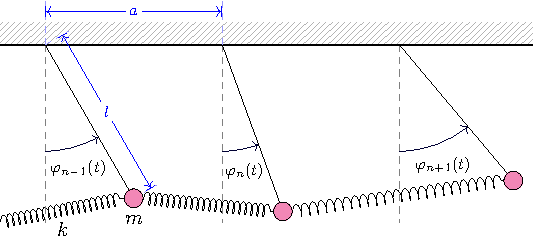
\includegraphics[scale=1.5]{img/osci_and_wave_in_ordered_struct/struct_of_pend}
	\label{fig:fig1}
\end{figure}

Обозначим $n$ -- номер маятника, $\omega_0^2=\frac{g}{l}$ -- собственная частота. Угол отклонения $n$-го маятника $\phi_n$, причем мы рассматриваем случай малых углов.


Состояние маятника зависит не только от времени $t$, но и от номера маятника $n$, то есть $n$ в некотором смысле играет роль пространственной координаты. Запишем уравнение динамики такого маятника:

\begin{equation}
	\ddot{\phi}_n+\omega^2_o \phi_n=\frac{\gamma}{m}\qty[\vphantom{\bigg|}(\phi_{n-1}-\phi_n)+(\phi_{n+1}-\phi_n)].
	\label{eq:1}
\end{equation}

Каждый маятник действует на соседние, причём сила взаимодействия зависит от разности значений углов. Упростим уравнение \eqref{eq:1}:

\begin{equation*}
	\ddot{\phi}_n+\omega^2_o \phi_n=\frac{\gamma}{m}\qty[\vphantom{\bigg|}\phi_{n-1}-2\phi_n+\phi_{n+1}].
\end{equation*}

Часто такую связь называют диффузионной, хотя, конечно, никакого отношения к процессу диффузии она не имеет. В системе нет диссипации, она линейна (нелинейность порождала бы новые частоты). Поэтому решение будем искать в следующем виде:
\begin{equation}
	\phi_n=A e^{i(\omega t-nka)}.
	\label{eq:2}
\end{equation}

Такая форма записи учитывает, что возмущение от маятника к маятнику проходит за некоторое конечное время.
\begin{equation}
	-\omega^2+\omega_0^2=\frac{\gamma}{m}\qty(e^{-ika}-2+e^{ika})
	\quad \Rightarrow \quad
	\omega^2=\omega_0^2-\frac{\gamma}{m}\qty(e^{-ika}-2+e^{ika})
	\label{eq:3}
\end{equation}
Рассмотрим случай  действительного $k$. Тогда
\begin{equation}
	\omega^2=\omega_0^2-\frac{\gamma}{m}(-2+2\cos{ka})=\omega_0^2+\frac{4\gamma}{m}\sin^2{\frac{ka}{2}}.
	\label{eq:4}
\end{equation}
Итак, мы установили, что $\omega$ и $k$ связаны соотношением \eqref{eq:4}. Построим график $\omega(k)$:
\begin{figure}[H]
	\centering
	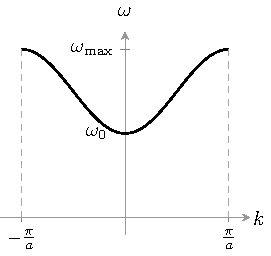
\includegraphics[scale=1.5]{img/osci_and_wave_in_ordered_struct/disp_of_struct}
\end{figure}
Нетрудно получить из уравнения \eqref{eq:4}, что 
\begin{equation*}
	\omega_{\max}=\sqrt{\omega_0^2+\frac{4\gamma}{m}}.
\end{equation*}
Если $\omega_0 < \omega < \omega_{max}$, то каждому $\omega$ соответствуют действительные $k_0$ и $-k_0$. Это означает, что каждой частоте соответствует две гармонические бегущие волны
\begin{equation*}
	\phi_n=A e^{i(\omega t+nk_0a)} 
	\qquad\text{и}\qquad
	\phi_n=A e^{i(\omega t-nk_0a)},
\end{equation*}
где $k_0$ -- волновое число. Поскольку система линейна, любая линейная комбинация решений тоже будет решением. 

Диапазон $\omega_0 < \omega < \omega_{\max}$ называют \textbf{полосой прозрачности} или полосой пропускания. Вне этой полосы решению не отвечают действительные $k$. В этом случае число \textit{$k$ - чисто мнимое} (чисто -- так как нет диссипации в системе) и $k=i\kappa$. Подставив такую связь в \eqref{eq:4}, получим
\begin{equation}
	\omega^2=\omega_0^2-\frac{4\gamma}{m}\sh^2{\frac{\varkappa a}{2}}.
	\label{eq:5}
\end{equation}
Подставляя \eqref{eq:5} в \eqref{eq:2}, получим вид волны в этом случае $\phi_n=A e^{-n\varkappa a} e^{i\omega t}$. Заметим, что при $n\rightarrow \infty$ функция  $\phi_n \rightarrow 0$, то есть в этих областях волна не проходит. 

Если мы находимся в полосе прозрачности, то $v_\text{фаз}=v_\text{фаз}(k), v_\text{фаз}=v_\text{фаз}(\omega)$. Если фазовая скорость зависит от частоты или волнового числа, то среда диспергирующая, а \eqref{eq:4} - дисперсионное соотношение. 

Дисперсия возникает из-за наличия собственных пространственных и временных масштабов : $a$ и $\omega_0$. У каждой компоненты волнового пакета будет своя фазовая скорость, возникнет его деформация. Именно наличием собственных масштабов объясняется то, что в одних случаях система пропускает волну, а в других нет.





\subsection{Предельный переход от цепочной структуры к среде}
Введём пространственную координату $x$ вдоль балки, на которой расположены точки подвеса. Сделаем замену, считая, что $\phi_n$ зависит от двух переменных:
\begin{equation*}
	\phi_n(t) \rightarrow \phi(x,t).
\end{equation*}
Считая $a$ малым, разложим $\phi_{n\pm 1}$ в ряд Тейлора по степеням $a$:
\begin{gather}
	\phi_{n+1}(t) \rightarrow \phi(x+a,t)=\phi(x,t)+\pdv{\phi}{x}a +\frac12 \pdv[2]{\phi}{x}a^2+\ldots,\\\nonumber
	\phi_{n-1}(t) \rightarrow \phi(x-a,t)=\phi(x,t)-\pdv{\phi}{x}a +\frac12 \pdv[2]{\phi}{x}a^2+\ldots
	\label{eq:6}
\end{gather}
Полученные разложеня до второго порядка подставим в \eqref{eq:1}:
\begin{gather*}
	\pdv[2]{\phi}{t} + \omega_0^2 \phi=\frac{\gamma}{m}a^2 \pdv[2]{\phi}{x}.
\end{gather*}
Обозначим $\frac{\gamma}{m}a^2 = v^2$, тогда уравнение  примет вид, известный как \textbf{уравнение Клейна-Гордона}:
\begin{equation}
	\pdv[2]{\phi}{t}-v^2\pdv[2]{\phi}{x}+\omega_0^2\phi=0.
	\label{eq:7}
\end{equation}
Уравнение \eqref{eq:7} не что иное, как уравнение в частных производных. Когда мы можем использовать \eqref{eq:7} вместо \eqref{eq:1}? Вспомним, что мы предполагали при решении задачи:
\begin{enumerate}
	\item Угол $\phi_n$, определенный в точке, определен и между дискретными точками подвеса;
	\item Отброшены величины третьего порядка;
	\item Расстояние между точками подвеса $a$ -- мало
\end{enumerate}

Построим дисперсионную характеристику для \eqref{eq:7}. Для этого подставим решение в виде бегущей волны в \eqref{eq:7}:
\begin{gather*}
	\phi(x,t)=Ae^{i(\omega t + kx)} \quad \Rightarrow \quad -\omega^2-k^2v^2+\omega_0^2=0,
\end{gather*}
\begin{equation}
	\omega^2 = \omega_0^2 + k^2v^2.
	\label{eq:8}
\end{equation}
\begin{figure}[H]
	\centering
	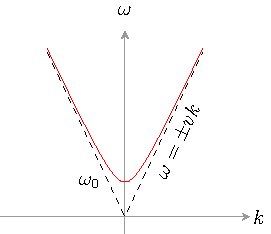
\includegraphics[scale=1.5]{img/osci_and_wave_in_ordered_struct/disp_of_cont}
\end{figure}
Нетрудно получить, что график имеет две асимптоты $\omega=\pm vk$. 

\paragraph{Условие совпадения дисперсионных соотношений. } При $\lambda\gg a$ или $ka\ll$ -- это условие длинноволновой зоны -- можно от соотношения \eqref{eq:4} перейти к \eqref{eq:8}. В этом случае пространственный масштаб не сказывается и мы им пренебрегаем. 

Если  $\omega_0 \rightarrow 0$, то из \eqref{eq:8} следует, что 
\begin{equation}
	\omega^2=k^2v^2.
	\label{eq:9}
\end{equation}
В этом случае система не обладает дисперсией:

\begin{figure}[H]
	\centering
	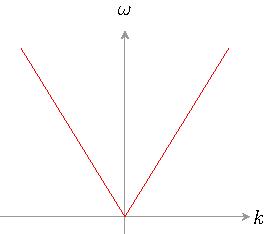
\includegraphics[scale=1.5]{img/osci_and_wave_in_ordered_struct/no_disp} 
\end{figure}

Дисперсионная характеристика проявляется в областях прозрачности или непрозрачности и зависимости $v_\text{фаз}$ от $k$ или $\omega$.

% Получили, шарики плотно друг к другу и покоятся.

Переход от цепочки к среде называется длинноволновым переходом: при нем теряется дискретность системы.




\subsection{Дисперсионное уравнение произвольной линейной системы}

Рассмотрим произвольную многомерную систему
\begin{equation}
	A\pdv{\vec{u}}{t}+B\pdv{\vec{u}}{x}+C\vec{u}=0
	\label{eq:10}
\end{equation}
Здесь $A, B, C$ --  матрицы размера $n\times n$, а $\vec{u}(x,t)$ описывает состояние системы. Будем искать решение в виде
\begin{equation}
	\vec{u}=\vec{\Psi} e^{i(\omega t - kx)}, \quad
	\vec\Psi=
	\begin{pmatrix}
		\Psi_1 \\
		\vdots \\
		\Psi_n \\
	\end{pmatrix}
	\label{eq:11}
\end{equation}
Подставляя \eqref{eq:11} в \eqref{eq:10}, получим
\begin{equation}
	Ai\omega\vec\Psi-iBk\vec\Psi+C\vec\Psi=0
	\quad \Rightarrow \quad
	(A\omega-Bk-iC)\vec\Psi i=0.
	\label{eq:12}
\end{equation}

Уравнение \eqref{eq:12} представляет собой систему линейных однородных уравнений относительно компонент вектора $\vec\Psi$. Она имеет решение, если ее детерминант равен нулю:
\begin{equation}
	\det\qty[A\omega-Bk-iC]=0.
	\label{eq:13}
\end{equation}

Для краткости это уравнение часто записывают в виде $D(\omega,k)=0$. Оно связывает $\omega$ и $k$, то есть задает дисперсионную характеристику. Следовательно, для $\forall k$ дисперсионное соотношение определяют $n$ значений $\omega$: $\omega_1(k), \dots, \omega_n(k)$. 

Каждой паре $k$, $\omega_s(k)$ отвечает некоторый вектор, определяемый \eqref{eq:12}. При этом решением будут не только $k, \omega, \vec\Psi$, но и комплексно сопряжённые $k^*, \omega^*, \vec\Psi^*$. Тогда можно построить действительное решение:
\begin{equation}
	\vec{u}(x,t)=\vec\Psi e^{i(\omega t-kx)}+\vec\Psi^* e^{-i(\omega^* t-k^*x)}.
	\label{eq:14}
\end{equation}
Уравнение \eqref{eq:14} задает гармоническую волну, если $k, \omega$ действительные. Если же $k, \omega$ комплексные, то \eqref{eq:13} задает нарастающее или затухающее колебание. При этом общее решение может быть записано в виде 
\begin{equation*}
	\vec{u}(x,t)=\sum_{s=1}^{n}\qty[ \Psi^{(s)}e^{i(\omega_s(k)t-kx)} + \text{к.с}.]
\end{equation*}

Как только мы учтём граничные условия для распределенной системы, получится аналог характеристических уравнений.




\newpage
\subsection{Влияние граничных условий}

% Рассмотрим несколько примеров постановки граничных условий в разных задачах.
% 
\paragraph{Кольцо из маятников.} Пусть маятники были свернуты в кольцо длины $L$ (см. рис. \ref{fig:figg}а). В силу того, что последний маятник является первым, $\phi_N = \phi_0$.

Подставляя граничное условие в решение, которые мы ищем $\phi_n = e^{i(\omega t - nka)}$, получим выражение для $k$
\begin{equation*}
	k=\frac{2\pi m}{L}, \quad m=1,2,3,\ldots
\end{equation*}
Следовательно, на длине кольца должно уложиться целое число волн.
% \begin{gather*}
% 	n=1,\dots,N;~~\phi_{n-1}-2\phi_n+\phi_{n+1}; \\
% 	k=\frac{2\pi n}{l};~~\phi_{N+1}=\phi_1;~~k=k_n.
% \end{gather*}	
\begin{figure}[H]
	\centering
	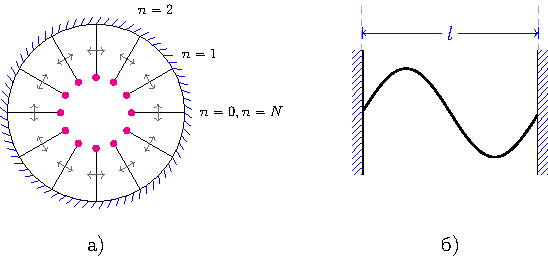
\includegraphics[scale=1.5]{img/osci_and_wave_in_ordered_struct/ring_of_pend}
	\caption{Различные динамические системы}
	\label{fig:figg}
\end{figure}

\paragraph{Закреплённая струна. } Примером распределенной системы может служить струна длины $l$, концы которой закреплены, а колебания описываются функцией $u(x,t)$ (см. рис. \ref{fig:figg}б). Граничное условие закрепления
\begin{equation*}
	u(0,t)=u(l,t)=0
\end{equation*}
Исходя из вида решения $u(x,t)=\Psi_1 e^{i(\omega t-kx)}+\Psi_2 e^{i(\omega t+kx)}$, получим условие укладывания целого числа полуволн:
\begin{equation*}
	\begin{cases}
		\Psi_1 e^{i\omega t}+\Psi_2 e^{i\omega t}=0 \\
		\Psi_1 e^{i\omega t}+\Psi_2 e^{i\omega t+ikl}=0
	\end{cases} \quad\Rightarrow\quad 
	\Psi_1=-\Psi_2,~~ \sin{kl}=0,~~ k=\frac{\pi m}{l}=k_m
\end{equation*}
Мы на нескольких примерах наблюдали, как наложение граничных условий приводит к дискретности спектра. 

Для характеристики произвольных линейных распределённых систем записывают систему
\begin{equation}
	\begin{cases}
		D(\omega,k)=0 \\
		k=k_n
	\end{cases}
	\label{eq:15}
\end{equation}

Отсюда при подстановке конкретных формул найдётся $\omega=\omega_n$. Если среда без дисперсии, то спектр волновых чисел и спектр частот будут эквидистантны. 





\subsection{Устойчивость состояний равновесия нелинейных распределенных систем}
Простейшим типом решений распределенных систем являются такие состояния, которые не меняются ни во времени, ни в пространстве: 
\begin{equation*}
	u=u_0 = \const
\end{equation*}
Будем их называть состояниями равновесия.

Уравнение, описывающее нелинейную распределенную систему, имеет вид
\begin{equation}
	\pdv{u}{t}=f\qty(u)+D\pdv[2]{u}{x},
	\label{eq:15}
\end{equation}
где $f(u)$ - нелинейная функция. Это уравнение реакции диффузии. Если убрать коэффициент диффузии $D$, то уравнение будет описывать динамику точки в среде. Мы рассмотрим  кубическую $f(u)$:
\begin{figure}[H]
	\centering
	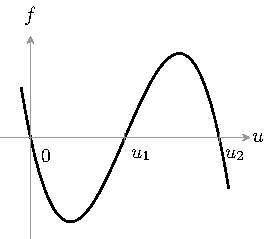
\includegraphics[scale=1.5]{img/osci_and_wave_in_ordered_struct/cub}
\end{figure}
В этом случае будет три точки, где $f(u)=0$. В системе могут быть стационарные решения $u=u_0(x)$ -- это другой тип решения. 

Будем изучать устойчивость решений для конкретного возмущения. Зададим возмущение в классе гармонических функций: 
\begin{equation*}
	\xi(x,t) = A e^{pt+ikx}
\end{equation*}
Линеаризуем \eqref{eq:16} на состояниях равновесия $u^*$, где $u=u^*+\xi(x,t)$:
\begin{equation}
	\pdv{\xi}{t}=D\pdv[2]{\xi}{x}+f'(u^*)\xi(x,t)
	\approx D\pdv[2]{\xi}{x}+f(u^*)+f'(u^*)\cdot\xi(x,t)
	\label{eq:16}
\end{equation}
Подставляя конкретный вид $\xi(x,t)$ и учитывая, что в состоянии равновесия $f(u^*)=0$, получим
\begin{gather*}
	p =-Dk^2+f'(u^*)
\end{gather*}


Проанализируем поведение системы в случае кубической $f(u)$, заданной ранее. В точках  $u=0$ и $u=u_2$ будет $f'(u^*)\hspace{-4pt}<\hspace{-4pt}0$, затухание возмущений. Значит, эти точки устойчивы. 



% Для каждого А.
\begin{figure}[H]
	\centering
	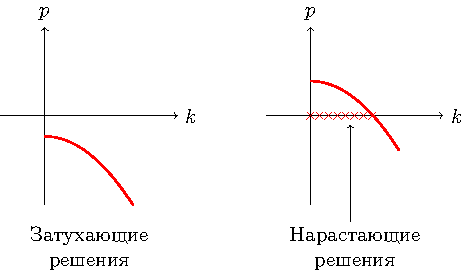
\includegraphics[scale=1.5]{img/osci_and_wave_in_ordered_struct/stability_or_instability} 
\end{figure}

В точке же $u_1$  производная $f'(u_1)>0$, значит, решение неустойчивое в классе возмущений $\xi(x,t)=A e^{pt+ikx}$.

Уравнение \eqref{eq:16}, в частности, описывает распространение пламени по бикфордовому (огнепроводному) шнуру. Волна превращает вещество из несгоревшего материала в сгоревшее.